% This is "sig-alternate.tex" V2.1 April 2013
% This file should be compiled with V2.5 of "sig-alternate.cls" May 2012
%
% This example file demonstrates the use of the 'sig-alternate.cls'
% V2.5 LaTeX2e document class file. It is for those submitting
% articles to ACM Conference Proceedings WHO DO NOT WISH TO
% STRICTLY ADHERE TO THE SIGS (PUBS-BOARD-ENDORSED) STYLE.
% The 'sig-alternate.cls' file will produce a similar-looking,
% albeit, 'tighter' paper resulting in, invariably, fewer pages.
%
% ----------------------------------------------------------------------------------------------------------------
% This .tex file (and associated .cls V2.5) produces:
%       1) The Permission Statement
%       2) The Conference (location) Info information
%       3) The Copyright Line with ACM data
%       4) NO page numbers
%
% as against the acm_proc_article-sp.cls file which
% DOES NOT produce 1) thru' 3) above.
%
% Using 'sig-alternate.cls' you have control, however, from within
% the source .tex file, over both the CopyrightYear
% (defaulted to 200X) and the ACM Copyright Data
% (defaulted to X-XXXXX-XX-X/XX/XX).
% e.g.
% \CopyrightYear{2007} will cause 2007 to appear in the copyright line.
% \crdata{0-12345-67-8/90/12} will cause 0-12345-67-8/90/12 to appear in the copyright line.
%
% ---------------------------------------------------------------------------------------------------------------
% This .tex source is an example which *does* use
% the .bib file (from which the .bbl file % is produced).
% REMEMBER HOWEVER: After having produced the .bbl file,
% and prior to final submission, you *NEED* to 'insert'
% your .bbl file into your source .tex file so as to provide
% ONE 'self-contained' source file.
%
% ================= IF YOU HAVE QUESTIONS =======================
% Questions regarding the SIGS styles, SIGS policies and
% procedures, Conferences etc. should be sent to
% Adrienne Griscti (griscti@acm.org)
%
% Technical questions _only_ to
% Gerald Murray (murray@hq.acm.org)
% ===============================================================
%
% For tracking purposes - this is V2.0 - May 2012

\documentclass{sig-alternate-05-2015}
%\usepackage{hyperref}
\usepackage{url}
\usepackage{listings}
\usepackage[utf8]{inputenc}

% Default fixed font does not support bold face
%\DeclareFixedFont{\ttb}{T1}{txtt}{bx}{n}{8} % for bold
%\DeclareFixedFont{\ttm}{T1}{txtt}{m}{n}{8}  % for normal

% Custom colors
\usepackage{color}
\definecolor{deepblue}{rgb}{0,0,0.5}
\definecolor{deepred}{rgb}{0.6,0,0}
\definecolor{deepgreen}{rgb}{0,0.5,0}
\definecolor{lightgrey}{rgb}{0.4,0.4,0.4}

% Python style for highlighting
\newcommand\pythonstyle{\lstset{
  language=Python,
  basicstyle=\scriptsize,
  breakatwhitespace=true,         % sets if automatic breaks should only happen at whitespace
  breaklines=true,                 % sets automatic line breaking
  captionpos=b,                    % sets the caption-position to bottom
  commentstyle=\color{lightgrey},    % comment style
  emph={},          % Custom highlighting
  emphstyle=\color{deepred},    % Custom highlighting style
  escapeinside={\%*}{*)},          % if you want to add LaTeX within your code
  extendedchars=true,              % lets you use non-ASCII characters; for 8-bits encodings only, does not work with UTF-8
  frame=tb,                         % Any extra options here around the code
  keepspaces=true,                 % keeps spaces in text, useful for keeping indentation of code (possibly needs columns=flexible)
  keywordstyle=\color{deepblue},
  otherkeywords={self, True, False},             % Add keywords here
  numbers=left,                    % where to put the line-numbers; possible values are (none, left, right)
  numbersep=5pt,                   % how far the line-numbers are from the code
  numberstyle=\tiny\color{lightgrey}, % the style that is used for the line-numbers
  rulecolor=\color{black},         % if not set, the frame-color may be changed on line-breaks within not-black text (e.g. comments (green here))
  showspaces=false,                % show spaces everywhere adding particular underscores; it overrides 'showstringspaces'
  showstringspaces=false,          % underline spaces within strings only
  showtabs=false,                  % show tabs within strings adding particular underscores
  stepnumber=1,                    % the step between two line-numbers. If it's 1, each line will be numbered
  stringstyle=\color{deepgreen},
  tabsize=1                  % sets default tabsize to 2 spaces
}}

% Python for external files
\newcommand\pythonexternal[2][]{{
\pythonstyle
\lstinputlisting[#1]{#2}}}

\begin{document}

% Copyright
%\setcopyright{acmcopyright}
%\setcopyright{acmlicensed}
%\setcopyright{rightsretained}
%\setcopyright{usgov}
%\setcopyright{usgovmixed}
%\setcopyright{cagov}
%\setcopyright{cagovmixed}


% DOI
%\doi{10.475/123_4}

% ISBN
%\isbn{123-4567-24-567/08/06}

%Conference
%\conferenceinfo{PLDI '13}{June 16--19, 2013, Seattle, WA, USA}

%\acmPrice{\$15.00}

%
% --- Author Metadata here ---
%\conferenceinfo{WOODSTOCK}{'97 El Paso, Texas USA}
%\CopyrightYear{2007} % Allows default copyright year (20XX) to be over-ridden - IF NEED BE.
%\crdata{0-12345-67-8/90/01}  % Allows default copyright data (0-89791-88-6/97/05) to be over-ridden - IF NEED BE.
% --- End of Author Metadata ---

\title{Development of a Search Engine and Applications in IR}
%
% You need the command \numberofauthors to handle the 'placement
% and alignment' of the authors beneath the title.
%
% For aesthetic reasons, we recommend 'three authors at a time'
% i.e. three 'name/affiliation blocks' be placed beneath the title.
%
% NOTE: You are NOT restricted in how many 'rows' of
% "name/affiliations" may appear. We just ask that you restrict
% the number of 'columns' to three.
%
% Because of the available 'opening page real-estate'
% we ask you to refrain from putting more than six authors
% (two rows with three columns) beneath the article title.
% More than six makes the first-page appear very cluttered indeed.
%
% Use the \alignauthor commands to handle the names
% and affiliations for an 'aesthetic maximum' of six authors.
% Add names, affiliations, addresses for
% the seventh etc. author(s) as the argument for the
% \additionalauthors command.
% These 'additional authors' will be output/set for you
% without further effort on your part as the last section in
% the body of your article BEFORE References or any Appendices.

\numberofauthors{4} %  in this sample file, there are a *total*
% of EIGHT authors. SIX appear on the 'first-page' (for formatting
% reasons) and the remaining two appear in the \additionalauthors section.
%
\author{
% You can go ahead and credit any number of authors here,
% e.g. one 'row of three' or two rows (consisting of one row of three
% and a second row of one, two or three).
%
% The command \alignauthor (no curly braces needed) should
% precede each author name, affiliation/snail-mail address and
% e-mail address. Additionally, tag each line of
% affiliation/address with \affaddr, and tag the
% e-mail address with \email.
%
% 1st. author
\alignauthor Robert Pinsler \\
       \affaddr{WKWSCI, NTU} \\
       \email{N1509281G@e.ntu.edu.sg}
% 2nd. author
\alignauthor Yiding Liu \\
       \affaddr{SCE, NTU} \\
       \email{LIUY0130@e.ntu.edu.sg}
% 3rd. author
\alignauthor Yitong Guan \\
       \affaddr{SCE, NTU} \\
       \email{GUAN0049@e.ntu.edu.sg}
\and  % use '\and' if you need 'another row' of author names
% 4th. author
\alignauthor Jenn Bing Ong \\
       \affaddr{SCE, NTU} \\
       \email{ONGJ0063@e.ntu.edu.sg}
}

% \date{30 July 1999}

\maketitle
\begin{abstract}
This study reports the development of a search engine that consists of indexing the dblp computer science bibliography data and process queries on the data fields in terms of keyword and phrase search. The relevance of the query results is evaluated and a user interface for the search engine is built. The most popular research topic and most similar publication venue and year are retrieved as part of the applications in information retrieval. 
\end{abstract}


%
% The code below should be generated by the tool at
% http://dl.acm.org/ccs.cfm
% Please copy and paste the code instead of the example below. 
%
\begin{CCSXML}
<ccs2012>
<concept>
<concept_id>10002951.10003317.10003347.10003349</concept_id>
<concept_desc>Information systems~Document filtering</concept_desc>
<concept_significance>500</concept_significance>
</concept>
<concept>
<concept_id>10002951.10003317.10003347.10003352</concept_id>
<concept_desc>Information systems~Information extraction</concept_desc>
<concept_significance>300</concept_significance>
</concept>
<concept>
<concept_id>10002951.10003317.10003359.10003361</concept_id>
<concept_desc>Information systems~Relevance assessment</concept_desc>
<concept_significance>100</concept_significance>
</concept>
</ccs2012>
\end{CCSXML}

\ccsdesc[500]{Information systems~Document filtering}
\ccsdesc[300]{Information systems~Information extraction}
\ccsdesc[100]{Information systems~Relevance assessment}

%
% End generated code
%

%
%  Use this command to print the description
%
\printccsdesc

% We no longer use \terms command
%\terms{Theory}

\keywords{Search engine; information retrieval; Lucene; DBLP; indexing; query processing; user interface}

% --------------------------------------------------------------------------------------------------------------------
\section{Introduction}
A search engine is an Information Retrieval (IR) system designed to help users find information stored on a computer system. In particular, a web-search engine is designed to search for information on the World Wide Web. The web was initially indexed by human until the 1990s when more and more web servers went online. Human-maintained lists are subjective and expensive to build and maintain, thus cannot scale the web effectively. It was not until a landmark paper by Google~\cite{Brin2012} that addresses both the issues of search quality and scalability of an automated web-search engine. Google introduced PageRank, uses the anchor text, proximity information, etc to improve the search quality dramatically and built a practical and automated web-search engine by fast crawling and query processing technology as well as robust database and operating system~\cite{Brin2012}.  

The web is a vast collection of completely uncontrolled heterogeneous documents; web documents have extreme variation both in terms of internal and external meta information. Big data refers to datasets that limits the capacity of traditional data processing systems to conduct effective analysis in terms of its data volume, quality, variety in data representation / structure, and acquisition speed; hence requiring new processing technologies~\cite{Chen2014}. All these add to the complexity of IR, which pose enormous challenge but presents unprecedented opportunity for new knowledge discovery in real-time that improves decision making. 

The objective of this study is to learn and practice the building blocks of a basic search engine using open-source Application Programming Interface (API) and applications in Information Retrieval (IR). The organization of this report is as follows. Recent development of search engine and IR are covered in Section 2. Section 3 provide information of the experimental setup such as dataset and API used. The results of the search engine built and IR applications are given in Section 4 with conclusion in Section 5.

% --------------------------------------------------------------------------------------------------------------------
\section{Recent Development}
\textit{\textbf{Elaborate on the recent development in search engine and information retrieval: personalised mobile search engine [...]}}
% --------------------------------------------------------------------------------------------------------------------
\section{Experimental Setup}
\textit{\textbf{Elaborate on DBLP dataset, Lucene API}}

\section{System Overview}

The search engine is able to index and search publication records listed in the dblp computer science bibliography (DBLP)~\cite{dblp}. It is built on top of PyLucene, a Python extension of the open-source software library Lucene\footnote{\url{https://lucene.apache.org}} that provides text indexing and search capabilities.

Publication records from DBLP are provided in a single XML file. The dataset comprises of various kinds of record types, such as articles published in a journal or magazine (\emph{article}), papers published in a conference or workshop proceedings (\emph{inproceedings}), books, and PhD theses. From those, only documents that are classified as \emph{article} or \emph{inproceedings} are considered.

\section{Indexing}

Indexing the DBLP dataset is a multi-step process. First, each record has to be extracted from the XML file before it can be further processed. Additional preprocessing is applied to match the expected input format. Finally, the records are processed and indexed through the PyLucene API. Listing \ref{lst:indexer} gives an overview of the Indexer class that provides above functionality. It takes as input the file to be indexed, the desired index storage location and an analyzer instance that we will introduce later. By calling its own index function, it triggers the indexing process (Listing \ref{lst:indexer}, line 12). In the following, we explain each step in more detail.

\lstset{caption={Indexer class}, label={lst:indexer}}
\pythonexternal{snippets/class_indexer.py}

\textbf{Parsing} \quad  We use an XML parser to extract the DBLP records from the dataset. Due to the large file size, reading in the whole XML tree at once is impractical. Instead, we use a SAX-like parser from the lxml\footnote{\url{http://lxml.de}} Python library that sequentially reads the document and emits events when it encounters certain XML tags. This allows to only react to \emph{<article>} and \emph{<inproceedings>} tags, thereby ignoring record types we are not interested in. This makes it very fast and memory-efficient. For each emitted event, we call the index\_document function. (Listing \ref{lst:indexer}, lines 15-19)

\lstset{caption={index\_document function}, label={lst:fn_index}}
\pythonexternal{snippets/fn_index.py}

\textbf{Preprocessing} \quad Given the current element, i.e. an \emph{article} or \emph{inproceedings} record, we can now iterate through its children, i.e. attributes of the record such as title or publication year. This is shown in Listing \ref{lst:fn_index}. As some of the records contain basic HTML formatting, irrelevant tags are removed and HTML-encoded characters are replaced  (Listing \ref{lst:fn_index}, lines 5 and 12-15).

\textbf{Indexing} \quad Each record is indexed as a Lucene \emph{document}, comprising of the following \emph{fields}: id, title, authors, year and venue. The venue is derived from the journal or booktitle attribute, depending on the record type. To facilitate the search, an additional \emph{content} field is added that concatenates the values of the above fields except the id. This can be easily achieved by subsequently adding all values to the same field. This method is also used to index multiple authors. (Listing \ref{lst:fn_index}, lines 19-20 and 27-28).

All fields are treated as strings\footnote{The \emph{year} attribute may also be stored as integer, allowing for features like range searches. However, this would require additional effort during search that we try to avoid.}. Contents of the original fields (i.e. without the \emph{content} field) are stored in the index, which allows to retrieve them later during search. This is especially useful to enhance search results with additional information when presented to the user. The values of the fields \emph{id} and \emph{year} are stored as-is, which is a property of the StringField class. All other fields are tokenized ($f_\text{token}$) and further processed. The processing applied to each of those TextFields is determined by the analyzer that is used, which is known by the index writer (Listing \ref{lst:indexer}, lines 6-10 and Listing \ref{lst:fn_index}, line 29). By default, all TextFields are processed in the same way, which may include lowercase conversion ($f_\text{low}$), removal of stopwords ($f_\text{stop}$) and stemming ($f_\text{stem}$). In particular, we use the Porter stemmer and the default stopword list of Lucene, which consists of 33 common English words.

Table \ref{tbl:analysis} summarizes the analysis applied to each field.

\begin{table}[th]
\centering
\caption{Analysis applied to document fields} \label{tbl:analysis}
\begin{tabular}{lcccc}
% \hline
Field & $f_\text{token}$ & $f_\text{low}$ & $f_\text{stop}$ & $f_\text{stem}$ \\
\hline
id & & & & \\
year & & & & \\
authors & X & X & X & \\
venue & X & X & X & \\
content & X & X & X & \\
title & X & X & X & X \\
% \hline
\end{tabular}
\end{table}

\textbf{Evaluation} \quad In order to evaluate the impact of additional token processing onto the index, different configurations of lowercase conversion, removal of stopwords and/or stemming are applied to the \emph{title} field. For this, we define a custom analyzer that gives us full control over the configurations by extending the base analyzer of PyLucene (Listing \ref{lst:customanalyzer}).

\lstset{caption={CustomAnalyzer class}, label={lst:customanalyzer}}
\pythonexternal{snippets/class_customanalyzer.py}

We measure the speed of indexing (including parsing and analyzing the documents) in seconds, $t_\text{ind}$, as well as the number of terms in the vocabulary, $|V_\text{title}|$. The results are shown in Table \ref{tbl:evalindex}. Note that indexing speed slightly varies over different runs.

\begin{table}[th]
\centering
\caption{Evaluation of token processing on \emph{title} field} \label{tbl:evalindex}
\begin{tabular}{cccrr}
% \hline
$f_\text{low}$ & $f_\text{stop}$ & $f_\text{stem}$ & $t_\text{ind}$ & $|V_\text{title}|$\\
\hline
& & & 417.97 ($100\%$) & 436\,354 ($100\%$) \\
X & & & 430.57 ($+3\%$) & 346\,286 ($-21\%$) \\
& X & & 414.89 ($-1\%$) & 436\,321 ($\pm0\%$) \\
& & X & 439.75 ($+5\%$) & 365\,534 ($-16\%$) \\
X & X & X & 417.94 ($\pm0\%$) & 288\,710 ($-34\%$) \\
% \hline
\end{tabular}
\end{table}

Applying lowercase conversion or stemming reduces the vocabulary significantly, whereas the removal of stopwords has nearly no impact. This is expected, since the first two techniques are able to map multiple tokens onto the same term whereas the exclusion of stopwords decreases the vocabulary size only by the number of stopwords. By combining multiple processing steps, the vocabulary can be further reduced, leading to a reduction of to up a third of the original size when no further processing is applied. In terms of indexing speed, we found that the additional processing steps are negligible. In particular, there seems to be no positive correlation between indexing speed and the number of processing steps that are applied. One reason for this is that while processing each document is more time-consuming, the cost for indexing a processed document is actually reduced. Therefore, we conclude that, under the given evaluation criteria, it is recommended to apply all three processing techniques due to the reduction in vocabulary size. However, it should be noted that this also has an effect on other properties of the system, e.g. the quality of search results, which might or might not be desired.

\section{Search}

\textbf{Keyword search} \quad The search module makes use of the document index to retrieve the most relevant documents to a given query. It supports free text keyword queries on any combination of the attributes title, authors, year and venue. By default, all attributes are considered. This is achieved by utilizing the \emph{content} field of the index. We refer to this as a standard search. Additionally, it is possible to query a combination of specific fields through an advanced search. Those keywords are directly matched against the respective fields in the index. In this case, documents must contain the provided keywords to be returned in the result set. Standard and advanced search can be freely combined during a single search request.

\textbf{Phrase queries} \quad Phrase queries are supported using double quotation marks (e.g. ``information retrieval'') in both standard and advanced search. Documents containing a particular phrase receive a higher weight during scoring. This requires an exact match up to the processing on the respective field. If a document does not contain the phrase, it may still be considered when there is a match for at least one of the keywords within the phrase. This considerably increases recall while risking an increase of false positives. Note that there is no restriction for the number of phrases within a query.

\textbf{Query results} \quad The search returns the $N$ most relevant documents along with their ranks, scores, ids and snippets, where $N$ is a configurable parameter. Relevance is determined based on Lucene's internal scoring function. It also measures the time needed to retrieve the results. The complete procedure for handling queries is outlined in Listing \ref{lst:search}.

\lstset{caption={Query handling},label={lst:search}}
\pythonexternal{snippets/search.py}

\section{Evaluation}

\section{User Interface}

There are two ways to interact with the search engine: via a text-based command line interface or via a web UI. The latter is built with Flask\footnote{\url{http://flask.pocoo.org}}, a leightweight Python web framework that leverages Jinja2\footnote{\url{http://jinja.pocoo.org}} as a templating engine. This allows to easily create HTML documents from within Python. Additionally, we incorporate the web framework Bootstrap\footnote{\url{http://getbootstrap.com}} to achieve responsive web design. Figure \ref{fig:search} depicts the search results for an example query. As the UI is not our focus, we omit further implementation details; the interested reader is referred to the source code.

\begin{figure*}[th]
\centering
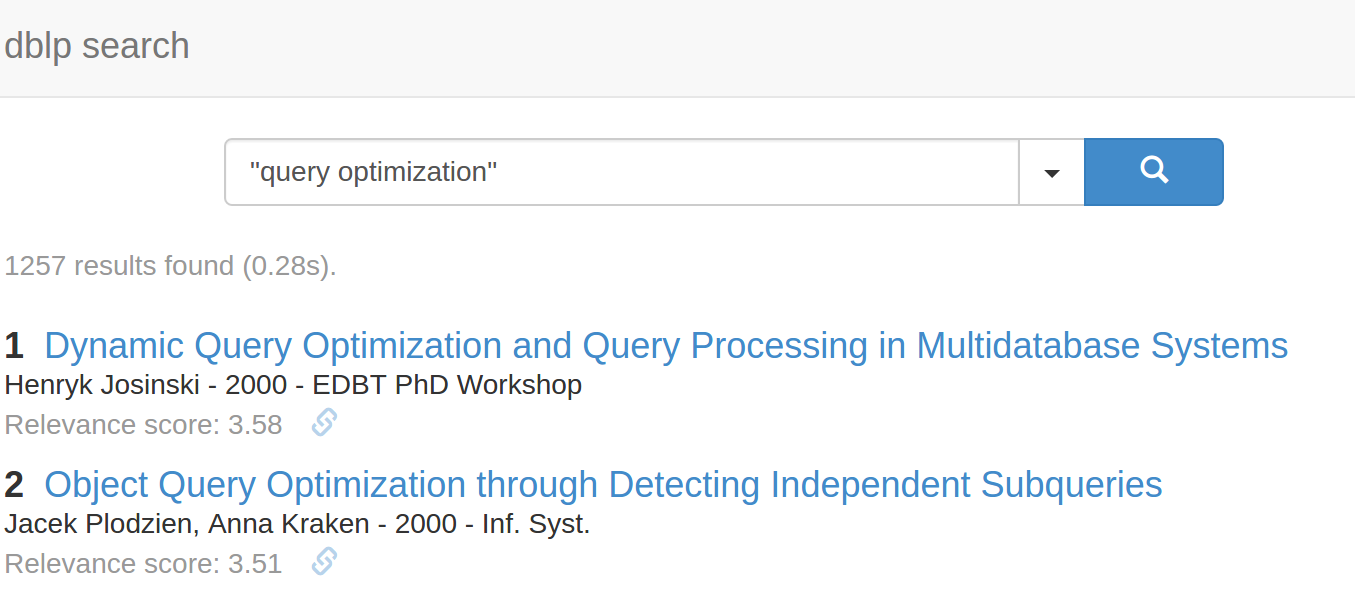
\includegraphics[width=.8\textwidth]{img/search}
\caption{Web-based search user interface}
\label{fig:search}
\end{figure*}

\section{Applications in IR}
We implement two applications based on dblp data. The first one is to find the top-10 most popular research topics of a specific year. The second one is finding top-10 similar publication venues and years with a given publication venue and year. Only paper titles are used in both application.

In this section, the related techniques and the detailed implementations of the applications are demonstrated, followed by the experiment results.

\subsection{Popular research topics}
Before mining popular research topics from paper titles, we need to firstly extract topics from such data. In our application, we identify meaningful topics from titles based on the patterns of words. More precisely, given a query (e.g. 2014), we have following process to extract topics from it:
\begin{itemize}
  \item Retrieve the titles of all the papers published in 2014, using the index.
  \item Tokenize each title and remove punctuations and stop words.
  \item Use Part-Of-Speech Tagger (POS Tagger)\footnote{\url{http://nlp.stanford.edu/software/tagger.shtml}} to assign parts of speech to each word, such as noun, verb, adjective, etc.
  \item Extract topics from the tagged words based on the given pattern, using regular expression tools.
\end{itemize}
The key point of topic extraction is the above steps is to define the word pattern of topic. From the observation of real topic names, we can conclude that
\begin{itemize}
  \item A topic name usually consist of adjectives and nouns.
  \item The adjectives always come before nouns for a topic name.
  \item Normally the number of words in a topic name is less than four.
\end{itemize}
Therefore, in the third step, we define the pattern as adj+adj+...+noun+...+noun. Moreover, only unigram, bigram and trigram are considered in this application. In addition, we ignore those unigram terms with very high (top 1\%) frequency because they may be some widely-used terminology in many different topics. After the topic identification, we count the frequency of each topic appeared in the titles. Finally, the top-10 most frequent topics will be return as the result.

\lstset{caption={Finding popular topics for a given year}, label={lst:popular_topics}}
\pythonexternal{snippets/popular_topics.py}

\subsection{Similar publication venues}
For retrieving similar publication venues and years, firstly we need to measure the similarity between two publication venues and years (e.g How similar are "TKDE'14" and "CIKM'15") using the paper titles. One simple way is to firstly tokenize every title of the venues and years, and use bag-of-words model, computing the cosine similarity of the word frequency vectors between them, which is defined as:
\begin{equation*}
  Sim_{i, j} = \frac{\sum_{k\in W}freq_{i,k} \cdot freq_{j,k}}{\sqrt{\sum_{k\in W}freq_{i,k}^2}\sqrt{\sum_{k\in W}freq_{j,k}^2}},
\end{equation*}
where i, j are two (venue, year) pairs. $W$ refers to the collection contains all the words appeared in the corpus. $freq_{i,k}$ is the frequency of word $k$ appears in the $i$th venue and year.

However, based on our statistical analysis, the dimensionality is too high. It is very inefficient to compute similarity. Besides, the data may also be very noisy, containing many words that only appears once in the whole dataset.

To address the aforementioned problems, we adopted Latent Dirichlet allocation (LDA)\cite{blei2003latent} to learn the latent topics from the data. Instead of using word frequency vectors, the similarity is defined based on the cosine similarity between the topic distribution of two venues and years. Thus, for a query venue and year, we compute the topic similarities between it and every other venues and years, which is given by

\begin{equation*}
  Sim_{i, j} = \frac{\sum_{z\in Z}\theta_{i,z} \cdot \theta_{j,z}}{\sqrt{\sum_{z\in Z}\theta_{i,z}^2}\sqrt{\sum_{z\in Z}\theta_{j,z}^2}},
\end{equation*}
where Z is the topic set; $\theta_{i,z}$ is the probability of the $i$th venue and year belongs to topic $z$.Then, based on the similarity, top-10 similar venues and years are returned as the result.

\begin{figure}[th]
\centering
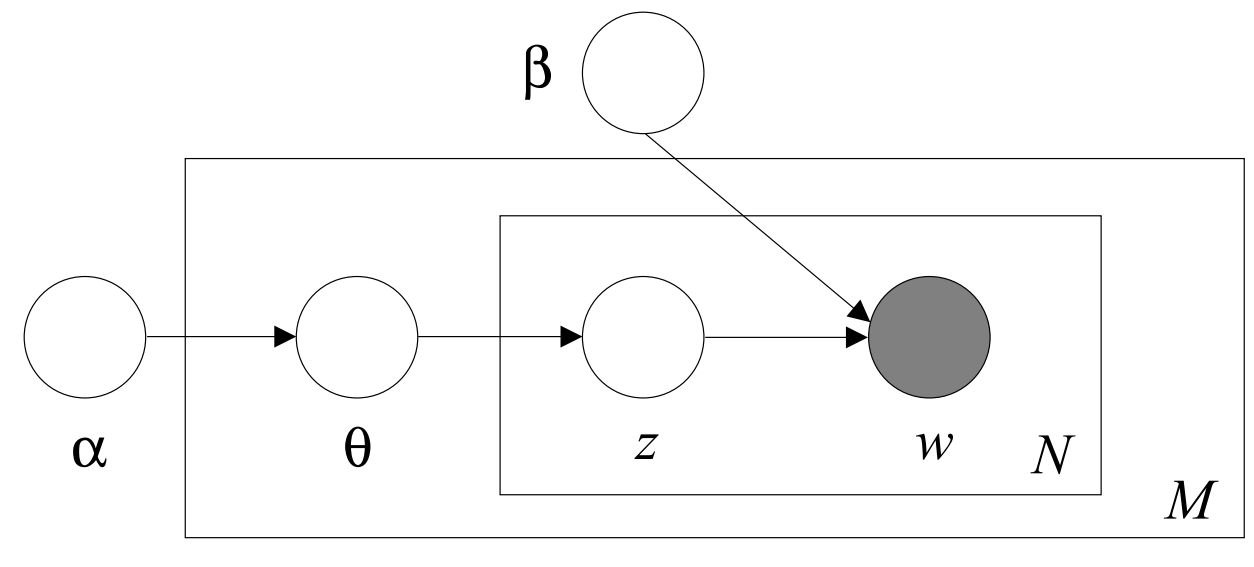
\includegraphics[width=0.48\textwidth]{img/LDA}
\caption{Graph representation of Latent Dirichlet allocation (LDA)}
\label{fig:lda}
\end{figure}

\begin{table}
\centering
\caption{Top-10 most popular research topics of the papers published in 2013} \label{tbl:app1}
\begin{tabular}{|c|c|c||c|} \hline
Rank & Topic & Frequency\\ \hline
1 & wireless sensor networks & 1412 \\ \hline
2 & case study & 1182 \\ \hline
3 & performance analysis & 568 \\ \hline
4 & cognitive radio networks & 468 \\ \hline
5 & special issue & 452 \\ \hline
6 & performance evaluation & 404 \\ \hline
7 & cloud computing & 373 \\ \hline
8 & genetic algorithm & 341 \\ \hline
9 & empirical study & 340 \\ \hline
10 & neural network & 340 \\ \hline
\end{tabular}
\end{table}

\begin{table}\small
\centering
\caption{Representive words for the topics leant by LDA} \label{tbl:topics}
\begin{tabular}{|p{65pt}|p{180pt}|} \hline
Topic & Words\\ \hline
Geographic Information System & data using based sar spatial sensing analysis remote images radar model land image satellite surface detection gis classification resolution hyperspectral \\ \hline
Robotics & robot control based using robots mobile motion robotic planning human autonomous design navigation vision dynamic sensor multi force tracking visual \\ \hline
Wireless Sensor Networks & networks wireless based network mobile routing ad hoc sensor protocol performance control using traffic efficient scheme qos algorithm 802 multi \\ \hline
Software Technology & software testing analysis based using test engineering development study code case model systems java quality source empirical tool approach program \\ \hline
Social Media & social online media networks community network behavior use internet effects study analysis communities understanding games self role game impact influence \\ \hline
\end{tabular}
\end{table}

\begin{table}
\centering
\caption{Top-10 most similar venues \& years to ``IEEE Trans. Knowl. Data Eng. 2014''} \label{tbl:app2}
\begin{tabular}{|c|c|c||c|} \hline
Rank & Venue & Year & Similarity\\ \hline
1 & IEEE Trans. Knowl. Data Eng. & 2015 & 0.9898 \\ \hline
2 & IEEE Trans. Knowl. Data Eng. & 2012 & 0.9888 \\ \hline
3 & DaWaK & 2015 & 0.9887 \\ \hline
4 & IEEE Trans. Knowl. Data Eng. & 2013 & 0.9856 \\ \hline
5 & LD4IE@ISWC & 2014 & 0.9850 \\ \hline
6 & CIKM & 2006 & 0.9845 \\ \hline
7 & WAIM & 2013 & 0.9830 \\ \hline
8 & CIKM & 2007 & 0.9823 \\ \hline
9 & FQAS & 2009 & 0.9815 \\ \hline
10 & CIKM & 2004 & 0.9803 \\ \hline
\end{tabular}
\end{table}

\subsection{Application Experiments}
For retrieving popular research topics, we have the results as follows:

For finding similar publication venues and years, we firstly learn the topics as follows:

The results of the queries are given as:
\section{Conclusions}

%
% The following two commands are all you need in the
% initial runs of your .tex file to
% produce the bibliography for the citations in your paper.
\bibliographystyle{abbrv}
\bibliography{report}  % sigproc.bib is the name of the Bibliography in this case
% You must have a proper ".bib" file
%  and remember to run:
% latex bibtex latex latex
% to resolve all references
%

\end{document}
